\documentclass{article}
\usepackage{circuitikz}
\usepackage{amsmath}
\usepackage[margin=1.5in]{geometry}
\usepackage{float}
\usetikzlibrary{matrix,arrows.meta,positioning}


\begin{document}
    \title{Chainship - Architecture}
    \author{Filip Krawczyk}
    \maketitle

    \section{Introduction}

    

    \section{Game logic}

    \subsection{Game state}

    \begin{figure}[H]
        \centering
        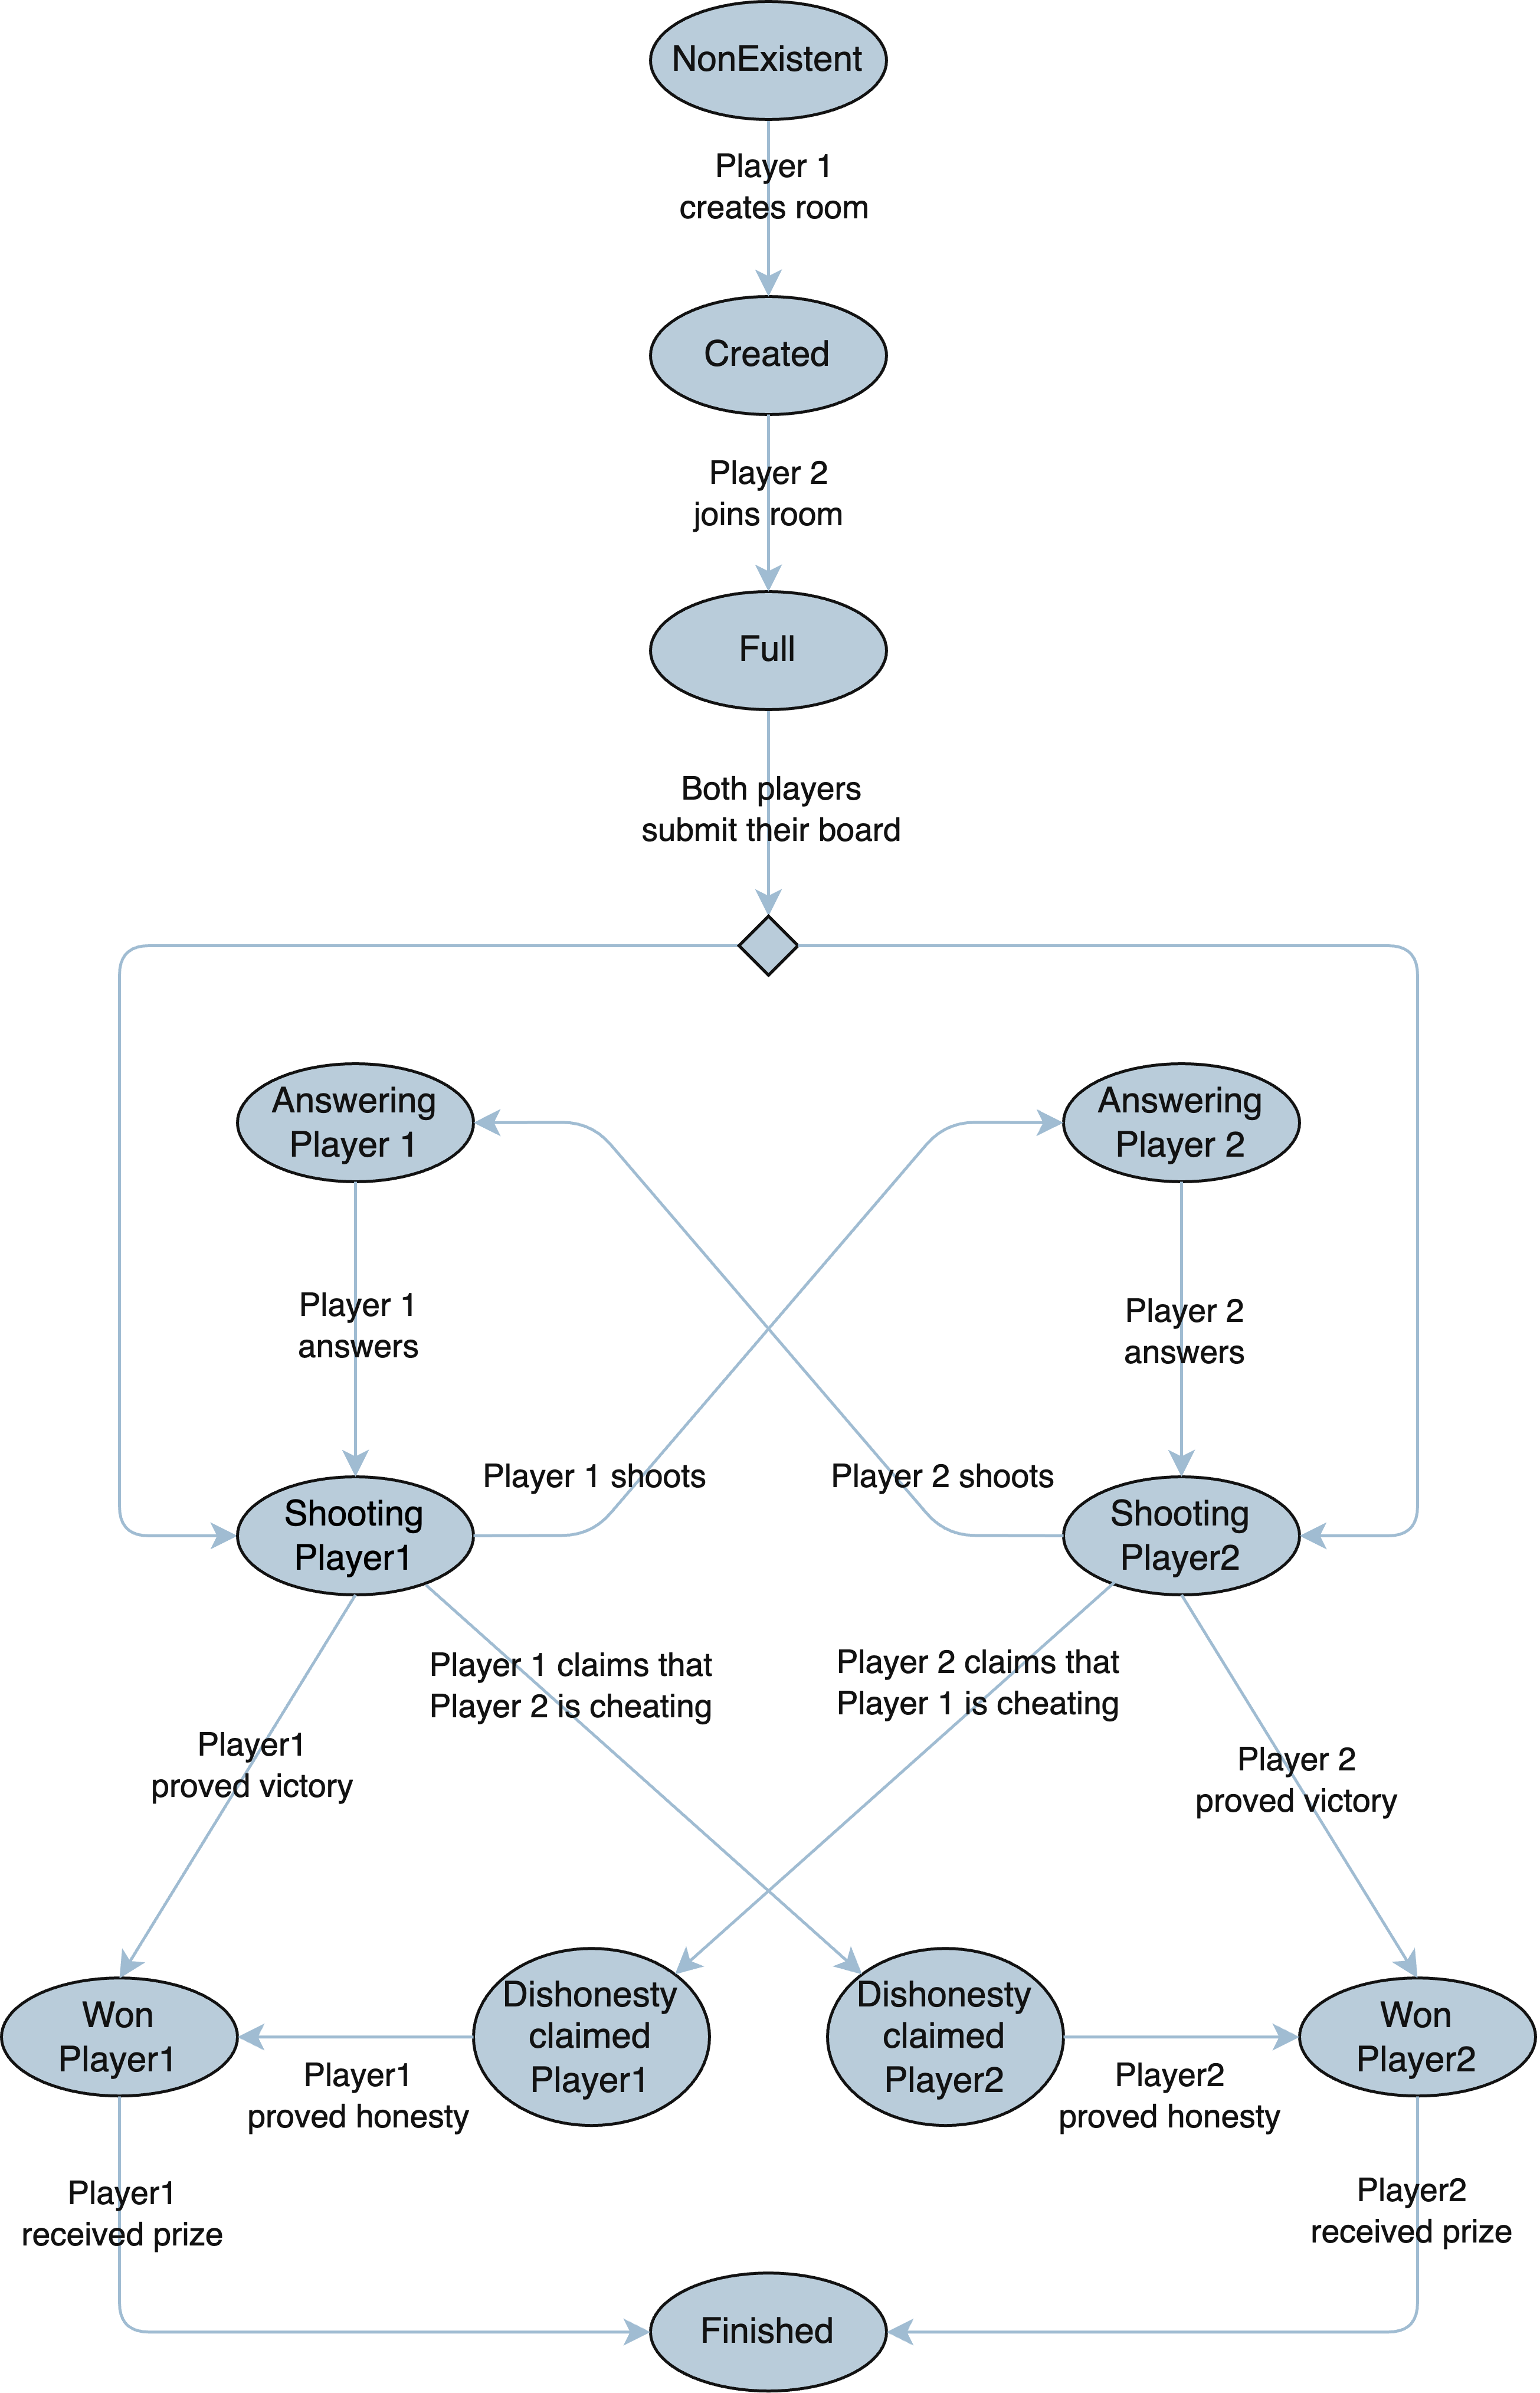
\includegraphics[width=0.75\textwidth]{state.png}
        \caption{Game state}
        \label{fig:game_state}
    \end{figure}

    \subsection{Randomizing first shooter}

    Since draw is not allowed, randomizing first shooter is crucial.

    \subsection{Proof of victory}

    Players can win in three ways:
    \begin{enumerate}
        \item Sinking all enemy ships.
        \item Showing that the opponent didn't answer correctly to shots.
        \item Enemy didn't answer in given time.
    \end{enumerate}
    To prove correct answers, the player has to provide decommitment to their board, list of answers and list of enemy's shots. Then, the contract checks if following criteria are met:
    \begin{enumerate}
        \item Board commitment was correct
        \item List of answers hashes to value stored in a contract
        \item List of enemy's shots hashes to value stored in a contract
        \item All answers were correct, given the board.
    \end{enumerate}
    Additionally, when proving victory, every enemy's ship has to be hit.

    \section{Cryptography}

    \subsection{Board commitment}
    Board is a $n \times n$ grid of cells. Each cell can be either empty or occupied by a ship. Players commit to the whole board before shooting stage begins. We define:

    \[ \operatorname{BoardHash}(b) = \operatorname{keccak256}(b_{1,1}, b_{1,2}, \ldots, b_{1,n}, b_{2,1}, b_{2,2}, \ldots, b_{2,n}, \ldots, b_{n,1}, b_{n,2}, \ldots, b_{n,n}) \]
    where $b_{i,j}$ is a boolean value that is true if there is a ship in cell $(i,j)$ and false otherwise.
    \\

    For small boards, it is easy to compute board hash for every possible board and therefore it wouldn't hide ships location. Because of that, randomness is introduced and board commitment is defined as follows:

    \[ \operatorname{BoardCommitment}(b,r) = \operatorname{keccak256}(\operatorname{BoardHash}(b) \; || \; r) \]

    \subsection{Shots hash}

    To reduce amount of data stored in a contract, shots are not stored directly. Instead, a single hash of all shots is stored. It is constructed in a way that makes it easy to iteratively compute it from previous hash and new shot.

    \begin{figure}[!ht]
        
        \centering
        \resizebox{1\textwidth}{!}{%
        \begin{circuitikz}
            \tikzstyle{every node}=[font=\LARGE]

            \draw  (1.25,13) rectangle (7.25,12);
            \draw [short] (4.25,13) -- (4.25,12);
            \draw [short] (5.75,13) -- (5.75,12);
            \node [font=\LARGE] at (2,12.5) {$h_0$};
            \node [font=\LARGE] at (3.5,12.5) {$1$};
            \node [font=\LARGE] at (5,12.5) {$x_1$};
            \node [font=\LARGE] at (6.5,12.5) {$y_1$};
            \draw (2.75,12) to[short] (2.75,13);
            \node [font=\LARGE] at (1.5,13.75) {};
            \draw [short] (4.25,12) -- (6.25,12);
            \draw [short] (4.25,12) -- (4.25,11.25);
            \draw [short] (4.25,11.25) -- (8.75,11.25);
            \draw [short] (8.75,11.25) -- (8.75,13.75);
            \draw [short] (8.75,13.75) -- (12,13.75);
            \draw [->, >=Stealth] (12,13.75) -- (12,13);
            \node [font=\LARGE] at (6.5,10.75) {keccak256};

            \draw  (11.25,13) rectangle (17.25,12);
            \draw [short] (14.25,13) -- (14.25,12);
            \draw [short] (15.75,13) -- (15.75,12);
            \node [font=\LARGE] at (12,12.5) {$h_1$};
            \node [font=\LARGE] at (13.5,12.5) {$2$};
            \node [font=\LARGE] at (15,12.5) {$x_2$};
            \node [font=\LARGE] at (16.5,12.5) {$y_2$};
            \draw (12.75,12) to[short] (12.75,13);
            \node [font=\LARGE] at (11.5,13.75) {};
            \draw [short] (14.25,12) -- (16.25,12);
            \draw [short] (14.25,12) -- (14.25,11.25);
            \draw [dashed] (14.25,11.25) -- (18.75,11.25);
            \draw [dashed] (18.75,11.25) -- (18.75,13.75);
            \draw [dashed] (18.75,13.75) -- (22,13.75);
            \draw [->, >=Stealth] (22,13.75) -- (22,13);
            \node [font=\LARGE] at (16.5,10.75) {keccak256};

            \draw  (21.25,13) rectangle (27.25,12);
            \draw [short] (24.25,13) -- (24.25,12);
            \draw [short] (25.75,13) -- (25.75,12);
            \node [font=\LARGE] at (22,12.5) {$h_{n-1}$};
            \node [font=\LARGE] at (23.5,12.5) {$n$};
            \node [font=\LARGE] at (25,12.5) {$x_n$};
            \node [font=\LARGE] at (26.5,12.5) {$y_n$};
            \draw (22.75,12) to[short] (22.75,13);
            \node [font=\LARGE] at (21.5,13.75) {};
            \draw [short] (24.25,12) -- (26.25,12);
            \draw [short] (24.25,12) -- (24.25,11.25);
            \draw [short] (24.25,11.25) -- (28.75,11.25);
            \draw [short] (28.75,11.25) -- (28.75,13.75);
            \draw [short] (28.75,13.75) -- (32,13.75);
            \draw [->, >=Stealth] (32,13.75) -- (32,13);
            \node [font=\LARGE] at (26.5,10.75) {keccak256};

            \draw  (31.25,13) rectangle (32.75,12);
            \node [font=\LARGE] at (32,12.5) {$h_n$};

            \end{circuitikz}
        }%

        \[ h_0 = 0 \]
        $ h_i = \operatorname{keccak256}(h_{i-1} \; || \; i \; || \; x_i \; || \; y_i) $ for $i \in \{ 1, 2, \ldots, n \}$
        \[ \operatorname{ShotsHash}(x_1, y_1, x_2, y_2, \ldots, x_n, y_n) = h_n \]
        
        \label{fig:shots_commitment}
    \end{figure}

    Obviously, hash $h_n$ is a function of all the shots $x_i$ and $y_i$ for $i \in \{ 1, 2, \ldots, n \}$, so given $h_n = \operatorname{ShotsHash}(x_1, y_1, x_2, y_2, \ldots, x_n, y_n)$ it is computationally infeasible to find different $(x'_i, y'_i)_{1 \leq i \leq n}$ such that $h_n = \operatorname{ShotsHash}(x'_1, y'_1, x'_2, y'_2, \ldots, x'_n, y'_n)$.

    The contraction of the commitment also makes it easy to compute the commitment for a new shot $(x_{n+1}, y_{n+1})$ given the previous commitment $h_n$ and the new shot. Smart contract only needs to store $i$ and $h_{i-1}$ for each player and whenever a new shot is made, it is broadcasted and the commitment is updated.

    \subsection{Answers hash}

    Hash of answers for shots is constructed in similar way except that answers $a_i$ are included in the hashed value, that is:
    \[ h_i = \operatorname{keccak256}(h_{i-1} \; || \; i \; || \; x_i \; || \; y_i \; || \; a_i) \]


\end{document}
